\chapter{Introduction à la programmation concurrente}\label{sec:into}
\startchapter

\section{Qu'est-ce que la programmation concurrente?}


\lettrine[lines=3]{E}{n} programmation séquentielle, un programme est décomposé en sous-programmes (procédures ou fonctions). Chaque sous-programme correspond à une suite d'instructions, et l'exécution du programme voit ces instructions être exécutées les unes à la suite des autres. Les premiers ordinateurs (et leurs successeurs durant quelques années) ont fonctionné selon ce mode d'exécution sérielle. Une tâche pouvait en appeler une autre, mais la tâche appelante ne continuait son exécution qu'après la terminaison de la tâche appelée. Cette approche, simple à mettre en oeuvre en comparaison des systèmes actuels, souffre toutefois de quelques faiblesses. Un seul programme peut être exécuté à la fois, ce qui interdit entre autres à un utilisateur de travailler sur un document en même temps qu'il compile un code source. Si le programme en cours d'exécution attend que l'utilisateur effectue une action (clic souris par exemple), alors le processeur se retrouve sous-exploité. Et enfin, si un programme engendre une erreur, et se fige, alors le système risque de se retrouver totalement bloqué.

À l'heure actuelle, les systèmes informatiques sont multiprocessus, et supportent l'exécution pseudo-parallèle de plusieurs processus (programmes en exécution). Ceci a été rendu possible par la mise au point de systèmes d'exploitation nettement plus complexes. Un processeur peut donc voir plusieurs processus en cours d'exécution se partager le temps de traitement. Et de même, un processus peut être décomposé en sous-processus ou \emph{tâche} (\emph{threads} en anglais). Ces threads permettent de ne plus être liés à une exécution totalement sérielle des instructions. Il est dès lors possible d'avoir, par exemple, un thread responsable d'exécuter un calcul lourd pendant qu'un autre gère les interactions avec l'utilisateur. Un serveur FTP, par exemple, peut plus facilement gérer plusieurs connexions simultanées, chaque connexion étant gérée par un thread.


\section{Parallélisme vs. concurrence}

Le terme \emph{programmation concurrente} ne doit pas être confondu avec celui de \emph{programmation parallèle} (ou programmation répartie). La programmation concurrente, telle que nous l'entendrons, se réfère à un système décomposé en tâches pouvant être exécutées dans un ordre quelconque. Certaines tâches sont exécutées avant d'autres, et certaines le sont en parallèle. La programmation parallèle traite, quant à elle, de l'exécution simultanée de tâches sur différents processeurs. Il s'agit alors de pouvoir synchroniser des processus entre eux, ceci principalement au travers d'une mémoire partagée ou de liaisons réseau.

Dans le cadre de ce cours, nous ne traiterons pas de la communication interprocessus, mais bien de la communication intraprocessus. Un programme sera décomposé en threads, qui sont donc ses fils d'exécution pseudo-parallèles. Les problèmes qui vont nous intéresser sont donc le partage de données et la synchronisation entre threads. Il est intéressant de noter que le concept de programmation concurrente est autant valable sur un processeur simple cœur que sur un multicœur. Sur un simple cœur, les parties de threads s'exécutent tour à tour de manière transparente, et sur un multicœur, un réel parallélisme peut être observé, chaque cœur pouvant exécuter un ensemble de threads.

L'illustration de la programmation concurrente sera faite par le biais de 2 langages. Le premier, le langage C, n'offre dans sa définition aucun mécanisme concurrent. Pour contourner ce problème, nous allons utiliser la bibliothèque standard \emph{pthread}, qui propose un ensemble de mécanismes pour la gestion des threads. Elle permet de décrire une application sous forme d'un ensemble de threads, ces threads étant ensuite exécutés sur la machine cible. Le second langage, Java, quant à lui, met à disposition la notion de threads et quelques mécanismes rudimentaires. Ce langage ne sera pas traité dans ce cours.

\section{Anatomie d'un processus}

Un processus correspond à un fichier exécutable en cours d'exécution sur un processeur. Il est entre autres caractérisé par un code (le programme à exécuter), une pile et un tas qui permettent de stocker les données nécessaires à son bon fonctionnement, un identifiant unique, et une priorité. La priorité permet au système d'exploitation de gérer plusieurs processus en cours d'exécution sur un processeur, un processus à plus haute priorité se voyant attribuer un temps d'utilisation de processeur plus important.

Un processus est créé lorsqu'un autre processus lance son exécution. Nous pouvons distinguer le processus parent (celui qui lance), et le processus enfant.

La figure \ref{fig:process-state-unix} illustre les différentes étapes de la vie d'un processus, pour un système d'exploitation de type Unix. L'état initial d'un processus est \emph{terminé} (\emph{destroyed} en anglais). Après sa création, il passe à l'état \emph{prêt} (\emph{ready} en anglais) lorsque toutes les ressources à son bon fonctionnement ont été réquisitionnées.
Le système d'exploitation peut ensuite le faire passer dans l'état \emph{élu}, (\emph{active} en anglais), état dans lequel le processus s'exécute.
Ce passage n'est pas du ressort du processus, mais bien de l'ordonnanceur, qui s'occupe d'allouer le processeur aux différents processus concurrents. À tout instant l'ordonnanceur peut replacer le processus dans l'état \emph{prêt}, pour laisser un autre processus s'exécuter. Il s'agit de la \emph{préemption} d'un processus, qui se fait sans que le processus préempté n'en soit conscient. Depuis l'état \emph{élu}, le processus peut aussi se retrouver dans l'état \emph{bloqué} (\emph{blocked} en anglais), lors de l'attente d'un événement ou du relâchement d'un mutex, par exemple. Il n'y a ensuite qu'une possibilité pour sortir de l'état \emph{bloqué}. Il s'agit de réveiller le processus suite au relâchement d'un mutex ou au fait qu'un événement sur lequel le processus attend a été déclenché. Dans ce cas, le processus passe à l'état \emph{prêt}, prêt à continuer son exécution. Lorsque le processus s'exécute, il peut se terminer. Les deux autres flèches sortantes de l'état \emph{élu} représentent deux scénarios. Premièrement, si le processus a été détaché, c'est-à-dire qu'il est sans lien parental, lors de sa terminaison, le processus passe directement dans l'état \emph{terminé}. Deuxièmement, si la terminaison du processus est importante pour le reste de l'application, alors il passe dans l'état \emph{zombie} (\emph{zombied} en anglais). Il y reste jusqu'à ce que le processus parent effectue une \emph{jointure}, c'est-à-dire qu'il récupère les informations retournées par le processus en cours de terminaison.

\begin{figure}[ht]
  \centering
  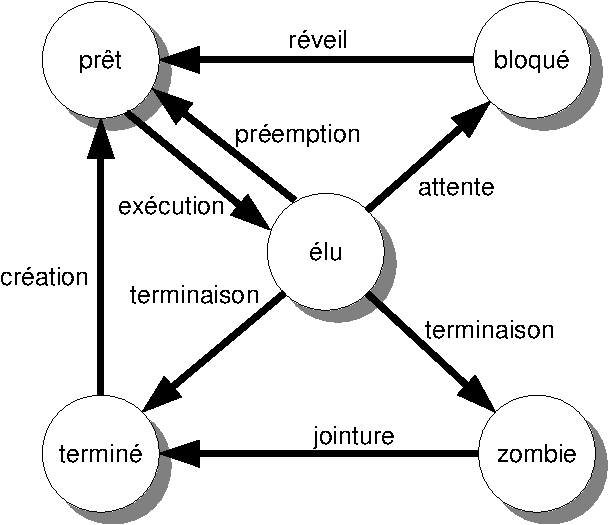
\includegraphics{images/process-state-unix}
  \caption{\label{fig:process-state-unix}États et transitions d'un processus Unix}

\end{figure}

La figure \ref{fig:process-space} illustre la décomposition de l'espace d'adressage d'un processus en trois parties principales~:
\begin{itemize}
  \item Le code contenant les instructions du programme (\emph{text segment} en anglais).
  \item Les variables globales et les variables allouées dynamiquement (\emph{data segment} en anglais).
  \item La pile, où les variables locales de ses sous-programmes, ainsi que diverses informations temporaires ayant une durée de vie égale au sous-programme sont stockées (\emph{stack segment} en anglais).
\end{itemize}

\begin{figure}[ht]
  \centering
  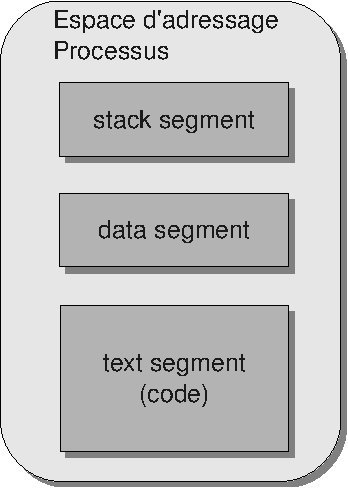
\includegraphics{process-space}
  \caption{\label{fig:process-space}Espace d'adressage d'un processus}

\end{figure}


Un processus, dans un cadre multithreadé, est décomposé en deux parties~:
\begin{itemize}
  \item La première contenant les ressources globales, telles que les instructions du programme et les variables globales. Cette partie correspond au \emph{processus}. Il s'agit des deux premiers points de l'espace d'adressage.
  \item La deuxième contenant des informations liées à l'état d'exécution, telles que le \emph{compteur de programme} (aussi appelé \emph{compteur ordinal}) et la \emph{pile d'exécution}. Cette partie correspond à un thread. Il est à noter que chaque thread possède un compteur de programme et une pile. Il s'agit de la partie liée au \emph{thread}.
\end{itemize}

\section{Anatomie d'un thread}

Un thread est un fil d'exécution de code, à l'intérieur d'un processus, et qui a la possibilité d'être ordonnancé. Il s'agit d'une version allégée d'un processus. Processus et threads partagent certaines propriétés, mais ne peuvent en aucun cas être interchangés. Tout processus a un thread principal, depuis lequel d'autres threads peuvent être lancés, dans le cas d'une application multithread.

Les threads d'un même processus partagent le même espace d'adressage, comme illustré à la figure \ref{fig:process-space-multi}. Toutes les ressources du processus peuvent être accédées par tous les threads, ce qui n'est pas le cas entre deux processus distincts. Toutefois, chaque thread possède son propre compteur de programme (PC), un ensemble de registres, un état, et une pile. Les piles sont placées dans l'espace mémoire dédié aux piles, mais chaque thread possède sa propre pile. Les variables globales sont par contre partagées entre les threads.

\begin{figure}[!ht]
  \centering
  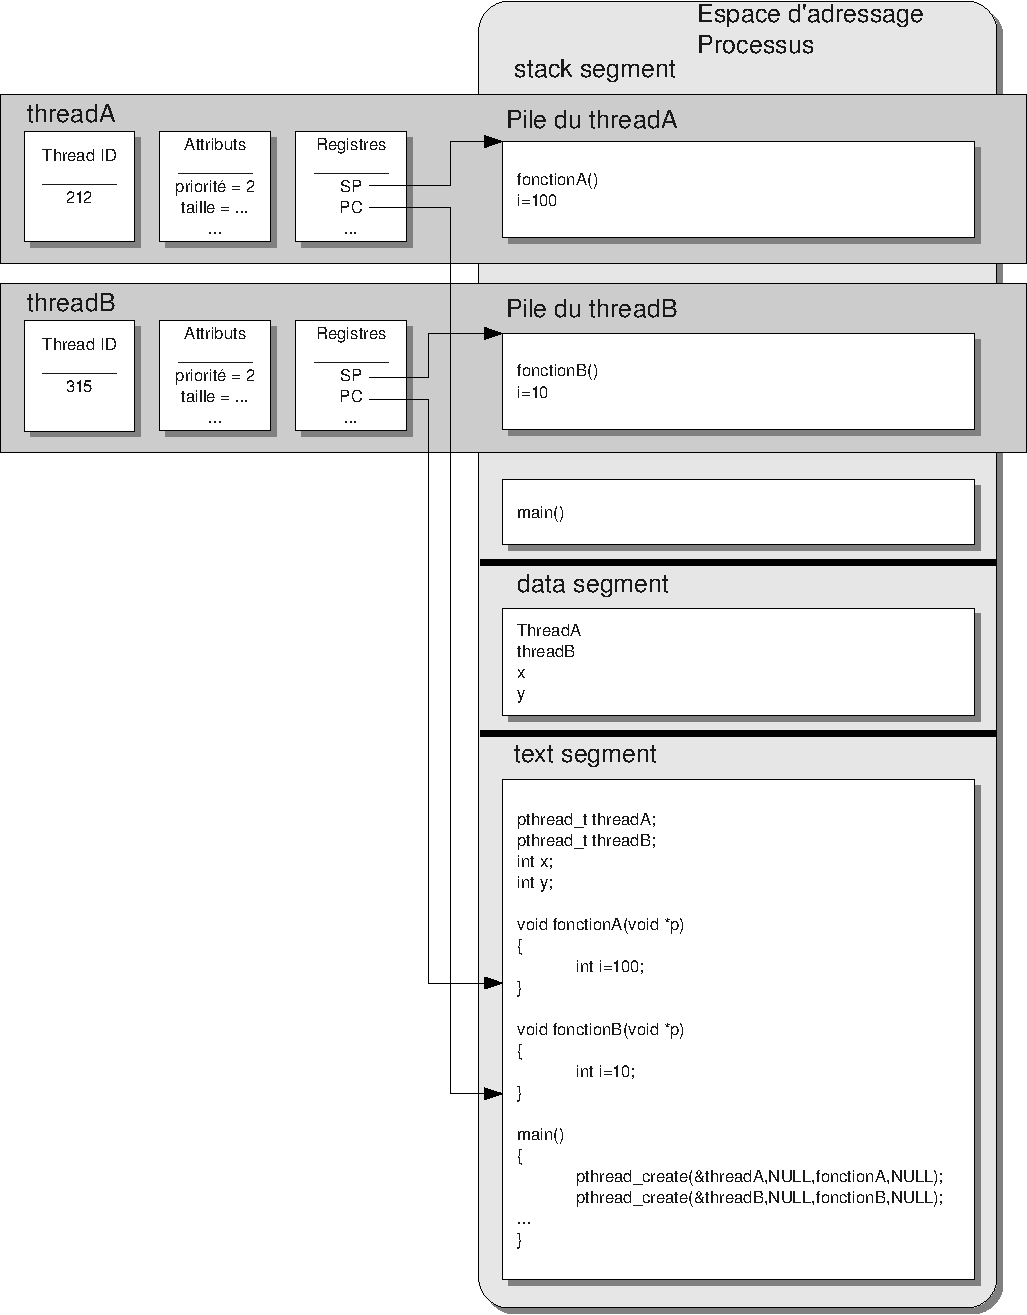
\includegraphics[width=\textwidth]{process-space-multi}
  \caption{\label{fig:process-space-multi}Espace d'adressage d'un processus multithread}

\end{figure}

Du point de vue du programmeur, le programme de la figure \ref{fig:process-space-multi} s'exécute à la manière présentée sur la figure \ref{fig:thread-execution}.

\begin{figure}[ht]
  \centering
  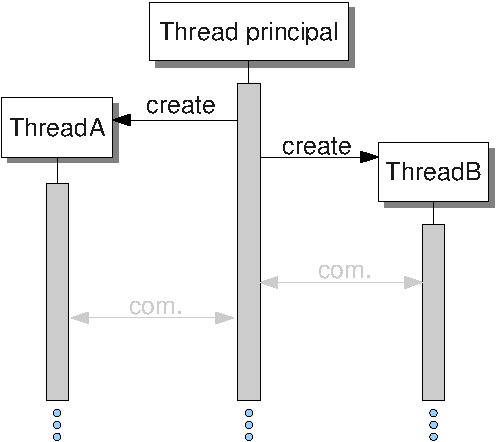
\includegraphics{thread-execution}
  \caption{\label{fig:thread-execution}Flot d'exécution d'un processus multithread}

\end{figure}

Toutefois, sur un processeur simple cœur, les threads doivent se partager le processeur. De ce fait, le flot d'exécution ressemble plutôt à celui présenté sur la figure \ref{fig:thread-execution-single}. Nous pouvons observer qu'un seul thread est en exécution à un instant donné, et que le passage d'un thread à un autre peut être influencé par une communication interthread (deux derniers cas), ou simplement dicté par l'ordonnanceur.

\begin{figure}[ht]
  \centering
  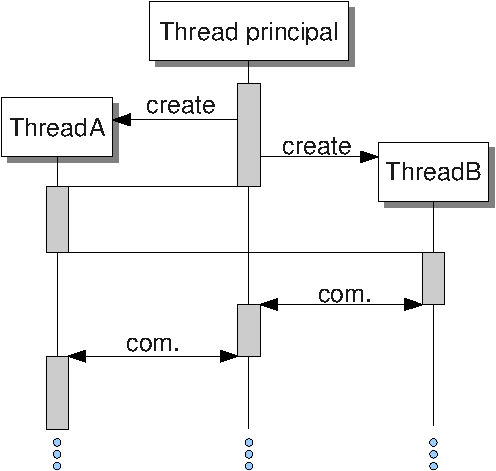
\includegraphics{thread-execution-single}
  \caption{\label{fig:thread-execution-single}Flot d'exécution d'un processus multithread sur un processeur simple cœur}

\end{figure}

Le cycle de vie d'un thread est semblable à celui d'un processus (figure \ref{fig:process-state-unix}).

Bien que la programmation multithread offre, dans le cadre de la programmation concurrente, passablement d'avantages sur la programmation multiprocessus, il faut être conscient des dangers y relatifs~:

\begin{itemize}
  \item Étant donné que les threads d'un même processus partagent le même espace d'adressage, un thread peut facilement corrompre les données utilisées par un autre thread. Des outils de synchronisation permettent toutefois d'éliminer les risques de ces corruptions, s'ils sont utilisés de manière appropriée.

  \item Toujours lié au partage de l'espace d'adressage, si un thread effectue un accès mémoire erroné fatal, le processus entier risque de se terminer. Ce n'est évidemment pas le cas pour un système à plusieurs processus.

  \item Un thread est lié à un programme particulier, et ne peut donc pas être lancé par un autre programme. Les processus peuvent en revanche être lancés par un autre processus, et donc être plus aisément réutilisés.
\end{itemize}

Pour résumer, listons ce que les processus et les threads ont en commun ou non.

En commun~:
\begin{itemize}
  \item possèdent un identifiant (ID), un ensemble de registres, un état, et une priorité;
  \item possèdent un bloc d'information;
  \item partagent des ressources avec les processus parents;
  \item sont des entités indépendantes, une fois créées;
  \item les créateurs du processus ou du thread ont contrôle sur eux;
  \item peuvent changer leurs attributs après création et créer de nouvelles ressources;
  \item ne peuvent accéder aux ressources d'autres threads et processus non reliés.
\end{itemize}

Pas en commun~:
\begin{itemize}
  \item les processus ont un espace d'adressage, les threads pas;
  \item les processus parents et enfants doivent utiliser des mécanismes de communication interprocessus; les threads d'un même processus communiquent en lisant et modifiant les variables de leur processus;
  \item les processus enfants n'ont aucun contrôle sur les autres processus enfants; les threads d'un processus sont considérés comme des pairs et peuvent exercer un contrôle sur les autres threads du processus;
  \item les processus enfants ne peuvent pas exercer de contrôle sur le processus parent; n'importe quel thread peut exercer un contrôle sur le thread principal, et donc sur le processus entier.
\end{itemize}


\section{Avantages du multithreading}

En comparaison d'un programme ne contenant qu'un seul thread, un programme décomposé en threads permet de mieux gérer les entrées/sorties et le calcul. Un thread peut s'occuper du calcul, tandis que d'autres gèrent les entrées/sorties. De ce fait, l'usage d'un GUI (Graphical User Interface) est plus ergonomique et convivial. Prenons l'exemple d'une application visant à afficher la courbe de Mandelbrot (Figure \ref{fig:mandelbrot}). Pour chaque point de l'image, une grande quantité de calcul doit être effectuée. Supposons que l'utilisateur peut cliquer sur des boutons pour zoomer. Si nous ne disposons pas de multithreading, un clic sur le bouton va ensuite voir l'application se bloquer pendant que la nouvelle image est calculée. Si par contre nous disposons de plusieurs threads, un thread peut s'occuper du calcul pendant que l'autre gère l'interface graphique. Dès lors l'utilisateur a encore la possibilité d'interagir avec l'application sans devoir souffrir de l'accaparement du processeur pour le calcul.

\begin{figure}[ht]
  \centering
  
\includegraphics[width=.7\textwidth]{mandelbrot_image}
  \caption{\label{fig:mandelbrot}Courbe de Mandelbrot}

\end{figure}

Dans le cas d'un processeur multicœur, un autre avantage du multithreading peut s'exploiter. En effet, chaque cœur peut prendre en charge un ou plusieurs threads. En reprenant l'exemple de Mandelbrot, si nous supposons que nous sommes en présence d'un dual-core, alors nous pouvons décomposer notre calcul en deux threads, chacun étant responsable de la génération de la moitié de l'image. Lorsque l'utilisateur clique sur le bouton, la nouvelle image pourra donc s'afficher en un temps réduit de moitié. Il s'agit là d'un parallélisme réel, rendu possible par l'amélioration des plateformes matérielles proposées sur le marché. Nous pouvons toutefois noter que l'accélération d'un facteur $n$ pour un $n$-core reste théorique, la probable communication interthread imposant une perte en performance.

En comparaison d'un système multiprocessus, une application multithread requiert une surcharge (overhead) moindre pour la gestion des tâches. En effet, commuter d'un thread à un autre est nettement moins coûteux en termes de temps processeur que de commuter d'un processus à un autre. Un avantage d'une application multiprocessus est la possibilité d'exécuter les processus sur des machines différentes, ce qui n'est pas le cas du multithread. Pour ce qui est de la commutation, le responsable de son fonctionnement, dans les deux cas, est le système d'exploitation.

La table suivante (tirée de \cite{hughes03parallel}) liste les avantages et les inconvénients du multithreading par opposition au multi-processing~:

\begin{table}[ht]
  \begin{center}
    \caption{\label{tab:thread-vs-process}Avantages et inconvénients du multithreading par opposition au multi-processing}
    \begin{tabular}{p{.5\textwidth}p{.5\textwidth}}
      \toprule
      \textbf{Avantage des threads}                                         & \textbf{Désavantages des threads}                                            \\
      \midrule
      Moins de ressources nécessaires lors d'un changement de contexte      & Requiert des mécanismes de synchronisation lors d'accès mémoires concurrents \\
      Améliore le débit de traitement des données dans une application      & Peut facilement polluer l'espace d'adressage du processus                    \\
      Ne nécessite pas de mécanismes spéciaux de communication entre tâches & N'existe que dans un processus, et n'est donc pas réutilisable               \\
      Permet de simplifier la structure d'un programme                      &                                                                              \\
      \bottomrule
    \end{tabular}
  \end{center}
\end{table}

\section{Séparation d'un programme en plusieurs threads}

A priori, n'importe quelle application pourrait être réalisée à l'aide d'un seul thread. Toutefois, comme nous l'avons vu, cette approche est quelque peu limitée. Il faut alors se poser la question concernant la meilleure manière de décomposer une application. Nous pouvons identifier différents types de modèles, qui définissent la façon dont les threads interagissent entre eux:

\begin{itemize}
  \item Le modèle \emph{délégation} (\emph{boss-worker model} ou \emph{delegation model} en anglais)
  \item Le modèle \emph{pair} (\emph{peer model} en anglais)
  \item Le modèle \emph{pipeline} (\emph{pipeline model} en anglais)
\end{itemize}

\subsection{Modèle délégation}

Dans le modèle \emph{délégation} (Figure \ref{fig:model-boss-worker}), un thread principal s'occupe de répartir la charge de travail sur les threads travailleurs. Ce pourrait typiquement être le cas d'un serveur FTP où un thread attend des commandes et les délègue ensuite aux autres threads. La réalisation d'une application selon ce modèle peut se faire de deux manières.


\begin{figure}[ht]
  \begin{center}
    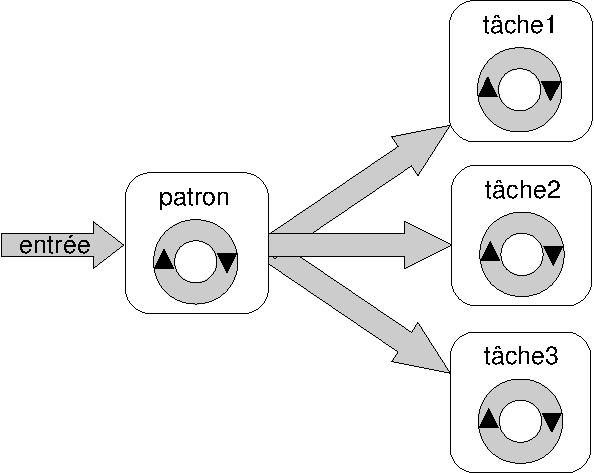
\includegraphics[scale=0.7]{model-boss-worker}
    \caption{\label{fig:model-boss-worker}Modèle délégation}
  \end{center}
\end{figure}

Premièrement, le thread principal peut créer un thread pour chaque nouvelle tâche à exécuter. Dans ce cas, il est composé d'une boucle dans laquelle il attend des requêtes et où il crée ensuite un thread capable de répondre à cette requête.

\newpage

\begin{codeblock}[list text={Exemple Patron},title={Exemple}]
void *patron(void *) {
  boucle infinie {
    attend une requête
    switch (requete) {
      case requeteX: pthread_create( ... tacheX); break;
      case requeteY: pthread_create( ... tacheY); break;
      ...
    }
  }
}

void *tacheX(void *) {
  exécuter le travail demandé, puis se terminer
}

void *tacheY(void *) {
  exécuter le travail demandé, puis se terminer
}
\end{codeblock}

Deuxièmement, le thread principal peut créer initialement un ensemble de threads. Il boucle ensuite en attendant une requête, et lorsqu'une requête arrive, la place dans une file d'attente. Tous les travailleurs sont également basés sur une boucle dans laquelle ils attendent qu'une requête soit placée dans la file d'attente. Un des travailleurs prend ensuite le contrôle de la requête et l'exécute.

\begin{codeblock}[list text={Exemple Travailleur},title={Un des travailleurs
prend le contrôle de la requête}]
void tacheX() { exécuter le travail demandé }
void tacheY() { exécuter le travail demandé }

void *patron(void *) {
  pthread_create(...);
  for (;;) {
    attend une requête;
    place la requête dans la file d'attente
    signale aux travailleurs qu'une requête est prête
  }
}

void *travailleur(void *) {
  for (;;) {
    bloque jusqu'à être activé par le patron
    récupère la requête de la file d'attente
    switch(requete){
      case requeteX: tacheX();
      case requeteY: tacheY();
      ...
    }
  }
}
\end{codeblock}

\subsection{Modèle pair}

Dans le modèle \emph{pair} (Figure \ref{fig:model-peer}), aucun thread n'est principal, tous étant égaux au niveau hiérarchique. Chaque thread est alors responsable de gérer ses propres entrées/sorties. La synchronisation entre thread risque fort d'y être nécessaire, afin que la tâche globale s'exécute correctement. Un exemple typique de ce type de modèle est une simulation d'un système physique décomposé en éléments finis. La modélisation de la chaleur dans une pièce, par exemple, pourrait voir le calcul être réparti entre plusieurs threads, chacun étant responsable d'une partie de la pièce. Le temps d'exécution d'une telle application sur une machine multicœur devrait alors être réduit. Il est toutefois à noter que la synchronisation nécessaire pour les interfaces entre les parties gérées par deux threads différents nécessite quelques précautions.


\begin{figure}[ht]
  \centering
  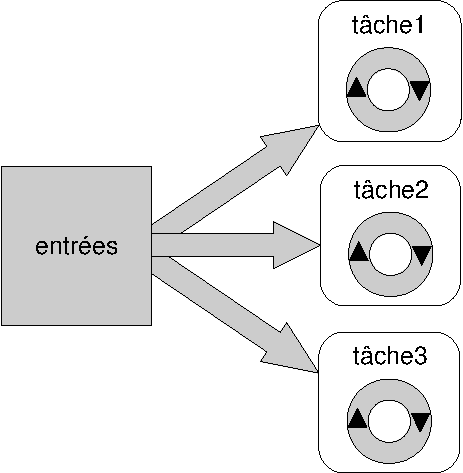
\includegraphics[scale=0.7]{model-peer}
  \caption{\label{fig:model-peer}Modèle pair}
\end{figure}


\begin{codeblock}[list text={Création Thread},title={Création de threads}]
task1() {
  attend le signal de commencement
  effectue le traitement, et synchronise avec les autres threads si nécessaire
}

task2() {
  attend le signal de commencement
  effectue le traitement, et synchronise avec les autres threads si nécessaire
}

main() {
  pthread_create( ... task1);
  pthread_create( ... task2);
  ...
  // signale aux threads qu'ils peuvent commencer à travailler
}


\end{codeblock}

\subsection{Modèle pipeline}

Le modèle \emph{pipeline} (Figure \ref{fig:model-pipeline}) est exploitable lorsque les conditions suivantes sont remplies:

\begin{itemize}
  \item L'application traite une longue chaîne d'entrée;
  \item le traitement à effectuer sur ces entrées peut être décomposé en sous-tâches (étages de pipeline) au travers desquelles chaque donnée d'entrée doit passer;
  \item chaque étage peut traiter une donnée différente à chaque instant.
\end{itemize}

\begin{figure}[ht]
  \centering
  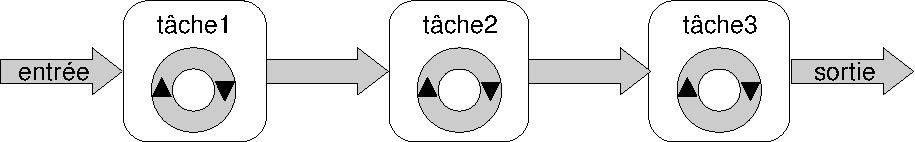
\includegraphics[scale=0.7]{model-pipeline}
  \caption{\label{fig:model-pipeline}Modèle pipeline}
\end{figure}


Là encore, un processeur multicœur devrait voir le temps d'exécution d'un programme grandement réduit. Un exemple typique permettant d'exploiter ce modèle serait du traitement sur un flux vidéo, où un étage modifierait la couleur, un autre le son, un autre appliquerait de la compression ...

Un étage du pipeline correspond donc à un traitement particulier à appliquer aux données. Le thread responsable de cet étage a un fonctionnement relativement simple. Il attend des données de l'étage précédent, traite ces données, et transmet ensuite le résultat de son traitement au thread responsable de l'étage suivant.

\begin{codeblock}[list text={Création Thread},title={Création de threads}]
floor1() {
  for(;;) {
    récupérer une entrée du programme
    traiter cette donnée
    passer le résultat à l'étage suivant
  }
}

floor2() {
  for(;;) {
    récupérer une donnée de l'étage précédent
    traiter cette donnée
    passer le résultat à l'étage suivant
  }
}

floorN() {
  for(;;) {
    récupérer une donnée de l'étage précédent
    traiter cette donnée
    passer le résultat en sortie du programme
  }
}

main() {
  pthread_create( ... floor1);
  pthread_create( ... floor2);
  ...
}
\end{codeblock}
